\subsection{Automated Reduction}
%\vspace*{-2ex}
We noticed that most of the useful feedback terms exist in the original query and hypothesized that the baseline system could be substantially improved by removing negative query terms. We used four approaches to refine the initial patent query: 
\begin{enumerate}
  \item removing document frequent terms (DF(t)>$\tau$),
 % \vspace*{-2ex}
  \item keeping frequent terms in query (QTF(t)>$\tau$),
  %\vspace*{-2ex}
  \item using pseudo relevance feedback to select query terms (PRF(t)>$\tau$), 
 % \vspace*{-2ex}
  \item removing general terms in IPC title. 
\end{enumerate}
In standard IR, removing terms, appearing a lot in the collection, helps the retrieval effectiveness. Inspired by this fact, we removed the words (in top-100 documents) with average term frequency higher than the threshold $\tau$ from the original query. As it can be seen in figure \ref{fig:queryreduc}, unlike our assumption, removing frequent terms in top-100 documents ($DF(t)>\tau$) ruined the performance.  

As mentioned in~\cite{maxwell2013compact} terms inside verbose queries are also important. Hence, we kept frequent words inside the query while removing document frequent words. The results in Figure \ref{fig:queryreduc} indicate that it is better to keep all query terms ($QTF(t)>\tau$). 

We used pseudo relevance feedback (PRF) as the third feature to reduce the query. PRF is an automated process without user interaction which assumes the top k ranked documents are relevant and the others are irrelevant. Again, it can be seen in Figure \ref{fig:queryreduc} that the results for query reduction using PRF were below the baseline. In fact, we could not find any heuristic correlates between  $ score_{RF}(t)$ and $ score_{PRF}(t)$. Figure \ref{fig:anecdotal} is an anecdotal example for a sample query which can explain the reason that PRF did not work. It shows the query abstract and a pair of PRF terms, with $ score_{PRF}(t)>10 $, and RF score of each term. It can be seen that terms with high PRF score have a negative RF score which means words from PRF contaminated with sufficient amount of noise to ruin the retrieval effectiveness. 
We used words in IPC code title to reduce the query because as it can be seen in Figure \ref{fig:queryreduc} the majority of them are negative terms as they are general words in all patents belonging to the same category. However we hurt the effectiveness by pruning them out.

Unlike our initial assumption, non of the standard proposed query reduction approaches for query reduction worked better than the baseline.
\begin{figure}
   \centering
   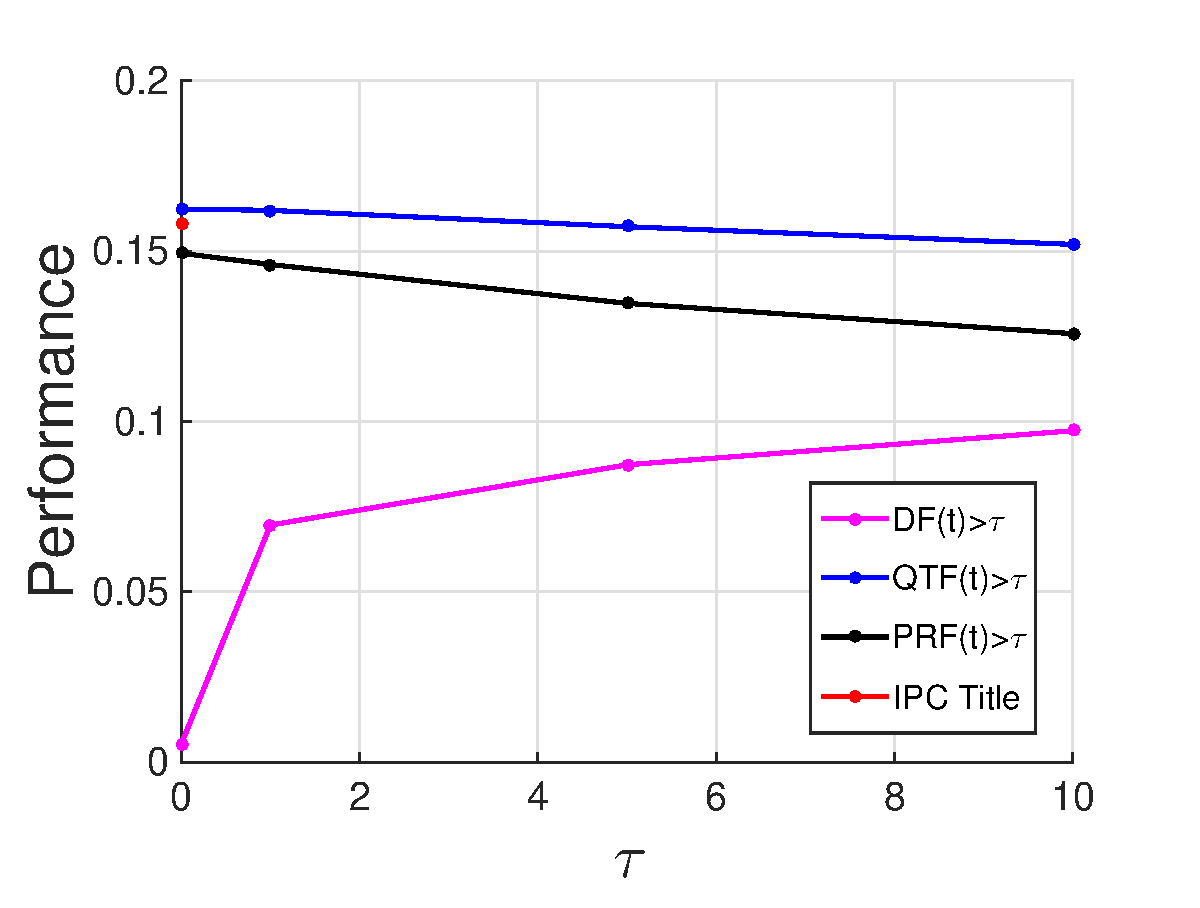
\includegraphics[width=0.35\textwidth,height=40mm]{figs/queryreduc-ipc.eps}
   \caption{System performance vs. the threshold $\tau$ for four query reduction approaches.}   
   \label{fig:queryreduc} 
\end{figure}

\begin{figure}[htpb]
\begin{framed}
\vspace*{-2ex}
  \centering
    %\lstinputlisting[frame=single, basicstyle=\scriptsize\ttfamily , linewidth=\columnwidth,breaklines=true]{code/anecdotale.tex}\vspace*{-2ex}
 \begin{lstlisting}[basicstyle=\scriptsize\ttfamily , linewidth=\columnwidth,breaklines=true] 
PAC-1293
Abstract: The invention relates to an emulsifier, 
a method for preparing said emulsifier, and to 
its use in various applications, primarily food 
and cosmetic applications. The invention also 
relates to the use of said emulsifier for the 
creation of an elastic, gelled foam. An 
emulsifier according to the invention is based on 
a starch which is enzymatically converted, using 
a specific type of enzyme, and modified in a 
specific esterification reaction.

DF Terms: <@\textcolor{blue}{starch:14.64}@>, <@\textcolor{blue}{enzym:29.49}@>, <@\textcolor{red}{amylos:-20.15}@>, 
<@\textcolor{blue}{oil:8.63}@>, <@\textcolor{red}{dispers:-8.66}@>, <@\textcolor{red}{ph:-4.55}@>, <@\textcolor{red}{dry:-6.21}@>, <@\textcolor{red}{heat:-2.26}@>, 
<@\textcolor{red}{product:-5.48}@>, <@\textcolor{red}{slurri:-11.48}@>, <@\textcolor{blue}{viscos:7.77}@>, <@\textcolor{red}{composit:-4.49}@>, 
<@\textcolor{red}{reaction:-1.97}@>, <@\textcolor{red}{food:-11.94}@>, <@\textcolor{blue}{agent:5.19}@>, <@\textcolor{red}{debranch:-10.58}@>, 
<@\textcolor{red}{reduc:-6.37}@>, <@\textcolor{red}{fat:-12.83}@>, <@\textcolor{red}{prepar:-0.82}@>, <@\textcolor{red}{hour:-5.42}@>, 
<@\textcolor{blue}{waxi:19.41}@>, <@\textcolor{blue}{deriv:11.97}@>, <@\textcolor{red}{content:-3.38}@>, <@\textcolor{blue}{aqueou:0.38}@>, 
<@\textcolor{red}{saccharid:-11.95}@>, <@\textcolor{red}{ml:-0.79}@>, <@\textcolor{red}{cook:-10.04}@>, <@\textcolor{blue}{modifi:5.65}@>, 
<@\textcolor{blue}{solid:5.50}@>, <@\textcolor{blue}{sampl:6.27}@>, <@\textcolor{blue}{mix:2.48}@>, <@\textcolor{red}{minut:-1.68}@>, <@\textcolor{red}{dri:-0.91}@>, 
<@\textcolor{red}{gel:-9.85}@>, <@\textcolor{blue}{activ:5.98}@>, <@\textcolor{red}{corn:-5.27}@>, <@\textcolor{blue}{alpha:12}@>, <@\textcolor{red}{sprai:-2.74}@> 

QTF Terms: <@\textcolor{blue}{starch:14.64}@>, <@\textcolor{blue}{emulsifi:6.72}@>, <@\textcolor{red}{succin:-3.46}@>, 
<@\textcolor{blue}{enzym:29.49}@>, <@\textcolor{blue}{emuls:12.66}@>, <@\textcolor{blue}{hydrophob:5.45}@>, <@\textcolor{red}{anhydrid:-5.47}@>, 
<@\textcolor{red}{reaction:-1.97}@>, <@\textcolor{red}{octenyl:-0.66}@>, <@\textcolor{blue}{stabil:3.64}@>, <@\textcolor{blue}{alkenyl:0.06}@>, 
<@\textcolor{blue}{reagent:1.17}@>, <@\textcolor{blue}{carbon:0.12}@>, <@\textcolor{blue}{potato:3.74}@>, <@\textcolor{red}{alkyl:-0.33}@>, 
<@\textcolor{red}{wt:-4.57}@>, <@\textcolor{blue}{ether:1.96}@>, <@\textcolor{red}{enzymat:-3.45}@>, <@\textcolor{blue}{convers:10.44}@>, 
<@\textcolor{red}{chain:-5.53}@>, <@\textcolor{blue}{atom:0.03}@>, <@\textcolor{red}{ph:-4.55}@>, <@\textcolor{red}{treat:-0.89}@>, 
<@\textcolor{red}{ammonium:-1.96}@>, <@\textcolor{red}{food:-11.94}@>, <@\textcolor{red}{amylos:-20.15}@>, 
<@\textcolor{red}{glucanotransferas:-0.86}@>, <@\textcolor{red}{glycidyl:-0.40}@>, <@\textcolor{red}{glycosyl:-0.02}@>, 
<@\textcolor{red}{dry:-6.21}@>, <@\textcolor{blue}{deriv:11.97}@>, <@\textcolor{blue}{transferas:0.89}@>, <@\textcolor{red}{foam:-0.49}@>, 

PRF Terms: <@\textcolor{blue}{starch:14.64}@>, <@\textcolor{blue}{encapsul:17.50}@>, <@\textcolor{red}{chees:-4.22}@>, 
<@\textcolor{blue}{oil:8.63}@>, <@\textcolor{blue}{hydrophob:5.45}@>, <@\textcolor{blue}{agent:5.19}@>, <@\textcolor{red}{casein:-2.19}@>, 
<@\textcolor{blue}{degrad:17.13}@>, <@\textcolor{blue}{deriv:11.97}@>, <@\textcolor{blue}{tablet:5.30}@>, <@\textcolor{red}{debranch:-10.58}@>, 
<@\textcolor{red}{imit:-1.13}@>, <@\textcolor{blue}{viscos:7.77}@>, <@\textcolor{blue}{oxid:5.97}@>, <@\textcolor{blue}{activ:5.98}@>, <@\textcolor{blue}{osa:9.32}@>, 
<@\textcolor{blue}{funnel:2.68}@>, <@\textcolor{blue}{amylas:26.06}@>, <@\textcolor{red}{amylopectin:-7.14}@>, <@\textcolor{blue}{maiz:20.61}@>, 
<@\textcolor{red}{blend:-3.17}@>, <@\textcolor{blue}{waxi:19.41}@>, <@\textcolor{blue}{convert:31.81}@>, 

IPC def Terms: <@\textcolor{blue}{cosmet:3.77}@>, <@\textcolor{blue}{toilet:0.18}@>, <@\textcolor{red}{prepar:-0.82}@>, 
<@\textcolor{blue}{case:0.47}@>, <@\textcolor{red}{accessori:-0.01}@>, <@\textcolor{red}{store:-0.37}@>, <@\textcolor{blue}{handl:0.07}@>, 
<@\textcolor{red}{pasti:-0.17}@>, <@\textcolor{red}{substanc:-1.21}@>, <@\textcolor{red}{fibrou:-0.01}@>, <@\textcolor{red}{pulp:-1.28}@>, 
<@\textcolor{red}{constitut:-0.06}@>, <@\textcolor{blue}{paper:1.26}@>, <@\textcolor{red}{impregn:-0.11}@>, <@\textcolor{blue}{emulsifi:6.72}@>, 
<@\textcolor{red}{wet:-0.28}@>, <@\textcolor{red}{dispers:-8.66}@>, <@\textcolor{red}{foam:-0.49}@>, <@\textcolor{red}{produc:-0.57}@>, 
<@\textcolor{blue}{agent:5.19}@>, <@\textcolor{blue}{relev:0.18}@>, <@\textcolor{blue}{class:0.053}@>, <@\textcolor{red}{lubric:-0.38}@>, 
<@\textcolor{blue}{emuls:12.66}@>, <@\textcolor{red}{fuel:-0.011}@>, <@\textcolor{blue}{deriv:11.97}@>, <@\textcolor{blue}{starch:14.64}@>, 
<@\textcolor{red}{amylos:-20.15}@>, <@\textcolor{red}{compound:-0.63}@>, <@\textcolor{red}{saccharid:-11.95}@>, 
<@\textcolor{blue}{radic:1.03}@>, <@\textcolor{red}{acid:-3.19}@> 
 \end{lstlisting} 
 \vspace*{-2ex}
\end{framed}
 \vspace*{-2ex}
  \caption{Anecdotal example: it shows the abstract, and $ t: \; RF(t) $ pair of a sample query, $\{t|DF(t)/QTF(t)/PRF(t)>10\}$. Useful terms are highlighted in blue and the noisy ones in red.}
  \label{fig:anecdotal}  
\end{figure}
\subsection{Reduction by Relevance Feedback}
All our attempts to improve the system effectiveness without accessing the relevance feedback were quite in vein because the features we recognized were tightly the combination of the useful words and noisy words and the system performance is too sensitive to the existence of a noisy word or the absence of the useful terms. So, we decided to apply much more realistic approach in which feedback terms are extracted only from the first ranked relevant document retrieved. Table \ref{tab:firstrel} shows that we can double the MAP by only the first-ranked relevant document.
\begin{table}[htpb]
  \begin{center}
   \caption{System performance using minimal relevance feedback. $\tau$ is RF score threshold, and $k$ indicates the number of first relevant retrieved patents.}\vspace{3mm}
  \input table/partialRFtermselect.tex   
  \label{tab:firstrel}
  \end{center}  
\end{table}
Fig. \ref{fig:FirstTPRankHisto} indicates that the baseline methods return a relevant patent, approximately, 80\% of the time in the first 10 results and 90\% of the time in the first 20 results, such an interactive approach requires relatively low user effort while achieving state-of-the-art performance.    
\begin{figure}[htpb]
   \centering
   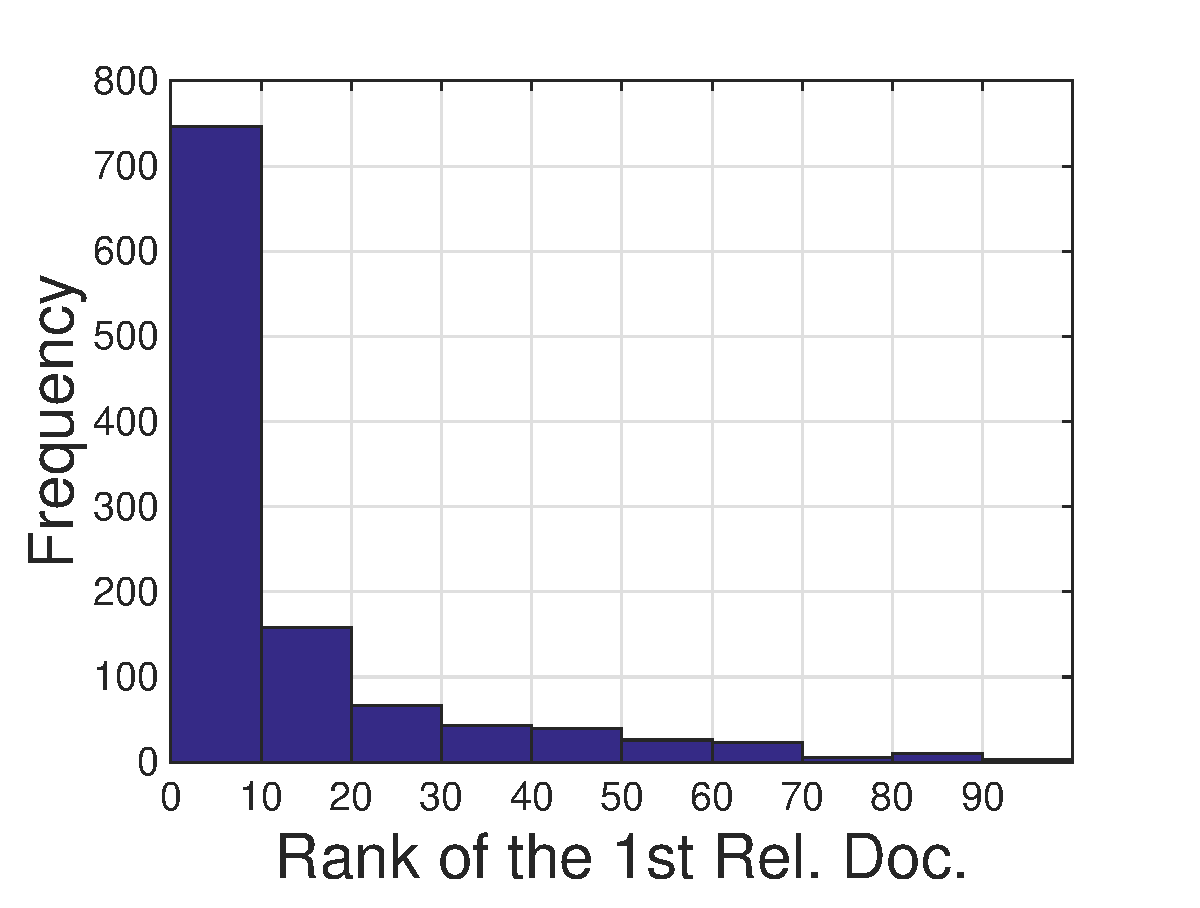
\includegraphics[width=0.25\textwidth,height=32mm]{figs/1stRank.eps}
   \caption{The distribution of the first relevant document rank over test queries}   
   \label{fig:FirstTPRankHisto} 
\end{figure}